\chapter{Analýza výsledků experimentů}

\section{Parametry simulátoru}
\label{sec:par_sim}
Ve všech experimentech jsme spouštěli simulace dopravy na dobu 5000 minut,
neboli simulovali jsme dobu 3 dny 11 hodin a 20 minut. Zvolili jsme střední hodnotu
času mezi výjezdy vozidla jako 0.1 minuty. Tedy každou minutu vyjede přibližně 10 nových 
vozidel. Jedna tato simulace běžela na stroji s procesorem AMD Ryzen™ 5 2500U 
\footnote{\url{https://www.amd.com/en/products/apu/amd-ryzen-5-2500u}} 
přibližně 4 minuty.

Silniční síť jsme si rozdělili na hrany délky 1 km (1 segment). Vzhledem
k úpravě ze \cref{sec:upravy} volíme vždy nejbližší nabíjecí stanici od aktuální
křižovatky (nevybíráme z množiny kandidátů). Spotřebu vozidla volíme jako 0.002
z celkové hladiny baterie za minutu a rychlost vozidla volíme jako 1 km/min (60 km/hod).
Tedy dojezd vozidla s maximální kapacitou je 500 km. 

Střední hodnotu normální distribuce popisující počáteční
hladinu baterie jsme zvolili jako 0.9 s rozptylem 0.2. Tuto volbu si můžeme odůvodnit
buď skutečností, že se vozidlo při výjezdu nestihlo nabít na plnou kapacitu. 
Předpokládáme, že doba nabíjení vozidla z domova trvá hodiny a v případě po sobě
jdoucích dlouhodobých cest v krátkém horizontu se baterie nemusí plně dobít.
Minimální výjezdová hladina baterie je zvolena jako 0.5. V simulátoru tedy mohou 
vyjíždět vozidla s počáteční hladinou v rozmezí 0.5 (dojezd 250 km) až 1 (dojezd 500 km).
V případě, že je odhadovaná hladina baterie v cílové destinaci menší než 0.05, pak
vozidlo také vyráží na nabíjecí stanici. Pokud je navíc hladina baterie menší než 0.5 
pak se vozidlo musí vždy rozhodnout zda vyrazí na nabíjecí stanici, či ne a od tohoto
okamžiku již nesmí změnit svou trasu do doby než dorazí do cílové destinace, či na 
nabíjecí stanici.

Dále volíme dobu čekání na úplné nabití vozidla jako 40 minut a každá nabíjecí
stanice má celkem 4 nabíjecí sloty (paralelně se můžou nabíjet 4 vozy).

V experimentech jsme porovnávali výsledky s následujími počty rozmístěných stanic:
100, 300, 500, 700, 1000, 2000, 4000

Vlastnosti simulátoru popisované výše nastavíme s pomocí následujících hodnot parametrů
(až na počet stanic všechny odpovídají základnímu nastavení parametrů programu):

\begin{Verbatim}
    "simulationTime" : [5000],
    "segmentLength" : [1],
    "numClosestStations" : [1],
    "carConsumption" : [0.002],
    "numStations" : [100, 300, 500, 700, 1000, 2000, 4000],
    "stationCapacity" : [4],
    "exponentialLambdaCities" : [0.005],
    "exponentialLambdaDepartures" : [10],
    "endCityRatio" : [1],
    "batteryTresholdLambda" : [20],
    "carBatteryMean" : [0.9],
    "carBatteryDeviation" : [0.2],
    "carStartBatteryBottomLimit" : [0.5],
    "chargingTreshold" : [0.5],
    "notChargingTreshold" : [0.9],
    "batteryTolerance" : [0.05],
    "carVelocity" : [1],
    "chargingWaitingTime" : [40],
    "meanChargingLevel" : [0.5]
\end{Verbatim}


\section{Parametry chybové funkce}
V chybové funkci, jež používáme pro optimalizaci, jsme zvolili parametr pro
počet stanic 100, pro počet vybitých vozidel také 100. Použití jedné nabíjecí
stanice tedy odpovídá vybití jednoho vozidla. Použítím těchto hodnot parametrů
zajistíme, že optimalizační algoritmy nebudou cíleně umísťovat velké množství
nabíjecích stanic jen za účelem eliminovat všechny vybité vozidla v simulaci.
Pokud by parametr pro počet nabíjecích stanic nebyl dostatečně velký, pak by 
optimální řešení bylo rozmístit nabíjecí stanici na každou možnou pozici, toto
řešení je však zjevně špatné a nerealistické. Naopak, pokud by byl parametr pro počet 
vybitých vozidel malý oproti počtu stanic, pak by nejoptimálnějším řešením
bylo nepoužít žádnou stanici bez ohledu na to, že se vybije velké množství vozidel.
Tento postup je však také zjevně špatný.

Parametr pro trvání cesty zanedbáváme, protože v simulátoru vhodně nepopisuje 
naši požadovanou hodnotu. Jeho hodnotu tak volíme jako 0.

Pro rozdíl hladin baterie volíme hodnotu 1 (nabývá hodnot z rozmezí -1 až 1, 
tedy ovlivní loss pouze minimálně). 

Parametr pro dobu čekání na nabíjecí slot
volíme jako 1, jelikož v optimálním řešení chceme, aby vozidla nečekala na nabíjecí 
stanici nerealisticky dlouho. Tato vlastnost však zjevně není stejně závažná 
jako počet stanic či vybitých vozidel, proto volíme hodnotu tohoto parametru poměrně malou.
Pro představu jedno vybité vozidlo považujeme za stejně závažnou závadu, jako
průměrné čekání vozidel 100 minut v řadě na nabíjecí slot. S ohledem na naše
nastavení počtu nabíjecích slotů slouží tento parametr pouze k eliminaci extrémních
případů (např. jediná nabíjecí stanice v řešení). Nepřipadá nám reálné, že se zvoleným
počtem stanic a počtem jejich nabíjecích slotů bude docházet k extrémně dlouhým čekacím dobám.

Parametry chybové funkce jsou tedy následující:

\begin{verbatim}
    "stationNumberParameter" : [100],
    "runDownParameter" : [100],
    "durationParameter" : [0],
    "batteryDifferenceParameter" : [1],
    "waitingTimesParameter" : [1]
\end{verbatim}

\section{Výsledky experimentů}
Kompletní výsledky experimentů a použité parametry lze nalézt v repozitáři práce v 
odpovídajících podadresářích (dle volby metody) v adresáři:

\begin{verbatim}
    final_version/analysis_results
\end{verbatim}

Nové parametry se nacházejí v adresářích s názvem (v odpovídajících adresářích 
optimalizačních metod, viz. předchozí odstavec):
\begin{verbatim}
    parameters1
\end{verbatim}

Nové výsledky experimentů lze nalézt v souborech s názvem (v odpovídajících adresářích 
optimalizačních metod):
\begin{verbatim}
    results1.txt
\end{verbatim}

\subsection{Náhodné rozmístění stanic}
Experimenty na modelech, v nichž jsme rozmísťovali nabíjecí stanice náhodně
stejný přístupem jako v případě generování počátečních pozic vozidel 
(pravděpodobnost počátečního města je závislá na počtu obyvatel, samotná pozice ve
městě je pak vygenerována uniformně nahodně), slouží především k porovnání náhodného 
přistupu vůči optimalizačním metodám a k otestování správného chování simulátoru.

Průměrný počet vybitých vozidel v simulacích (přes všechny zvolené počty stanic, jež
popisuje \cref{sec:par_sim}) je 2965.86. Průměrný počet vozidel, které dokončily 
svou cestu (dojezd do cíle a návrat do startu považujeme za 2 odlišné cestu) 
je 89872.9 a průměr vozidel, které nestihly dokončit svou trasu (simulace skončila), je
2252. Tyto počty přibližně korespondují s očekávaným počtem vozidel v simulaci, který je
50000 (připbližně 10 vozidel vyjede za 1 minutu) a celkově očekávaným počtem tras 100000
(každé vozidlo má naplánovány vždy 2 trasy (tam a zpět)). Vozidla, jež nedorazily
do cílové destinace (vybily se nebo nestihly dojet), mohly být ve na své první cestě (v budoucnu by
přispěly 2 krát do celkového počtu tras), nebo mohly být na cestě zpět do počátku 
(v budoucnu by přispěly jednou). Celkový počet tras vozidel při započtení nedokončených tras tedy
je v rozmezí 95091 a 100308. Toto rozmezí přibližně odpovídá
počtu očekávaných cest popsaných výše (asi 100000). Počet vybitých vozidel klesá s rotoucím počtem nabíjecích stanic
na mapě, počet dokončených cest naopak roste (očekávaný průběh).

Na počet vybitých vozidel lze nahlížet jako na počet neúspěšných cest do cílové destinace.
Neúspěšných cest do cílové destinace je tedy přibližně 3.2\%. Vzhledem k tomu, že ne všechny vozidla
vyrážejí s plnou kapacitou baterie (v nejhorším případě i s hladinou 0.5, tedy s dojezdem 250 km),
průměrná vzdálenost do cíle je 200 km (tedy s poměrně velkou pravděpodobností překračuje také vzdálenost 250 km)
a také, že může být nabíjecí stanice vzdálená (jejich pozice jsou náhodné), předpokládáme, 
že poměr vybitých vozidel a úspěšných cest rozumně
odpovídá vlastnostem simulovaného modelu. V neposlední řadě je třeba také do předpokládaného
počtu vybitých vozidel započítat počet vybití způsobených pouze aproximativní volbou nejvhodnější
nabíjecí stanice.

U průměrné doby čekání na nabíjecí slot nepozorujeme výraznou závislost na počtu stanic. Tuto 
skutečnost si odůvodňujeme dostatečně velkým počtem nabíjecích slotů na nabíječkách, který vede k malé
pravděpodobnosti přeplnění nabíjecí stanice (pravděpodobně by bylo možné celkový počet 
nabíjecích slotů na stanicích snížit).

Z pohledu využitelnosti stanic můžeme sledovat trend, že s rostoucím počtem narůstá počet stanic, jež
nebyly za celou dobu simulace použity. Pro porovnání v případě 100 umístěných stanic bylo využito 95 stanic.
V případě 4000 umístěných stanic však bylo použito pouze 1358 stanic.

Podrobné výsledky popisuje \cref{tab:vysledky_nahodne}.


\begin{table}
\centering\footnotesize\sf
\begin{tabular}{lrrrrr}
\toprule
$N$ & $R$ & $t$ & $F$ & $Not F$ & $N_{used}$ \\
\midrule
100 & 4104 & 4.28264 & 88361 & 2006 & 95  \\
300 & 3742 & 7.33916 & 89050 & 2092 & 259  \\
500 & 3377 & 7.58291 & 88679 & 2125 & 400  \\
700 & 3137 & 8.45333 & 89505 & 2218 & 522  \\
1000 & 2801 & 7.4205 & 90789 & 2239 & 643 \\
2000 & 2148 & 6.60937 & 90902 & 2538 & 982  \\
4000 & 1452 & 5.56316 & 91824 & 2546 & 1358 \\
\bottomrule
1228.57 & 2965.86 & 6.75015 & 89872.9 & 2252 & 608.429 \\
\end{tabular}
\caption{Výsledky simulace při náhodné rozmístění stanic a různých počtech umístěných stanic.
$N$ - počet umístěných stanic, $R$ - počet vybitých vozidel, $t$ - průměrný doba čekání na nabíjecí slot, $F$ - počet dokončených
cest vozidel (buď dojezd do cíle, nebo návrat do počáteční pozice), $Not F$ - počet vozidel, které nestihly
dokončit svou cestu (simulace doběhla), $N_{used}$ - počet nabíjecích stanic, využitých aspoň 1 vozidlem. Poslední
řádek tabulky vyobrazuje průměrné hodnoty.}
\label{tab:vysledky_nahodne}
\end{table}


\subsection{Optimalizační metody}
S ohledem na potřebu odevzdat analýzu výsledků co nejdříve, jsme bohužel byli nuceni
spouštět optimalizační metody na parametrech vyžadující kratší dobu výpočtu, což
je znatelné především u optimalizace genetickým algoritmem, která pracuje s malou populací
a malým počtem generací.

\subsubsection{Hladový algoritmus}
Pro optimalizaci hladovým algoritmem jsme použili rozdíl loss pro ukonční optimalizace
100, maximální počet iterací 5 a rozhodli jsme se porovnávat variantu, kdy 
odebíráme v každém kroku 1, 5 a 10 stanic. Parametry simulátoru jsou tedy:

\begin{verbatim}
    "lossDifferenceTreshold" : [100],
    "greedyMaxIterations" : [5],
    "greedyNumThrowAway" : [1, 5, 10]
\end{verbatim}


U této optimalizační metody očekáváme
zredukování počtu nabíjecích stanic s přibližným zachováním počtu vybitých vozidel oproti náhodnému řešení.
Z výsledků lze vypozorovat mírný pokles počtu vybitých vozidel oproti náhodné variantě (náhodná změna 
nepoužívaných stanic pravděpodobně mírně optimalizuje rozmístění stanic). Zajímavý je však znatelný pokles
v době čekání na stanicích, který je 4.75052 oproti 6.75015 v náhodné variantě. 
Toto zlepšení může být způsobeno výhodnějším rozmístěním pozic stanic.

Podrobnější výsledky hladové optimalizace viz. \cref{tab:vysledky_greedy}.

\begin{table}
\centering\footnotesize\sf
\begin{tabular}{lrrrrrr}
\toprule
$N$ & $R$ & $t$ & $F$ & $Not F$ & $N_{used}$ & $Num_{throw}$ \\
\midrule
97 & 3975 & 2.32103 & 88994 & 1936 & 97 & 10 \\
97 & 3964 & 2.39562 & 88236 & 1974 & 94 & 1 \\
100 & 4056 & 1.32837 & 88014 & 1948 & 98 & 5 \\
285 & 3651 & 2.3415 & 88275 & 1991 & 234 & 5 \\
300 & 3679 & 3.60535 & 89284 & 2035 & 254 & 1 \\
300 & 3662 & 3.58768 & 88867 & 2099 & 255 & 10 \\
480 & 3428 & 7.14107 & 88962 & 2110 & 337 & 5 \\
480 & 3440 & 3.1488 & 88733 & 2052 & 364 & 10 \\
500 & 3347 & 3.75678 & 88741 & 2045 & 400 & 1 \\
680 & 3169 & 4.50716 & 88417 & 2126 & 448 & 10 \\
700 & 3107 & 4.39188 & 89225 & 2132 & 511 & 5 \\
700 & 3177 & 4.34124 & 89255 & 2116 & 510 & 1 \\
995 & 2771 & 5.85256 & 89629 & 2303 & 570 & 5 \\
1000 & 2752 & 6.27729 & 89820 & 2178 & 640 & 1 \\
1000 & 2712 & 6.42694 & 89425 & 2214 & 647 & 10 \\
2000 & 2129 & 7.20114 & 91496 & 2428 & 992 & 5 \\
2000 & 2024 & 7.10672 & 91419 & 2391 & 997 & 1 \\
2000 & 2028 & 7.22709 & 91860 & 2441 & 994 & 10 \\
3960 & 1252 & 5.54454 & 92185 & 2702 & 1365 & 10 \\
3980 & 1293 & 5.66007 & 91998 & 2648 & 1360 & 5 \\
3996 & 1274 & 5.59811 & 92022 & 2751 & 1360 & 1 \\
\bottomrule
1221.43 & 2899.52 & 4.75052 & 89755.1 & 2220 & 596.524 & - \\
\end{tabular}
\caption{Výsledky hladové optimalizace.
$N$ - počet umístěných stanic, $R$ - počet vybitých vozidel, $t$ - průměrný doba čekání na nabíjecí slot, $F$ - počet dokončených
cest vozidel (buď dojezd do cíle, nebo návrat do počáteční pozice), $Not F$ - počet vozidel, které nestihly
dokončit svou cestu (simulace doběhla), $N_{used}$ - počet nabíjecích stanic, využitých aspoň 1 vozidlem, 
$Num_{throw}$ - počet stanic pro vyřazení v jedné iteraci hladové optimalizace. Poslední
řádek tabulky vyobrazuje průměrné hodnoty.}
\label{tab:vysledky_greedy}
\end{table}


\subsubsection{Genetický algoritmus}
V experimentech zkoumající genetický algoritmus jsme uvažovali velikost populace 10 jedinců,
počet generací 10 nebo 20, výběr do další generace buď 0 nebo 4 nejlepší jedince, pravděpodobnost
lepší volby v turnajové selekci 0.7 a 0.9, pravděpodobnost mutace stanice v jedinci 0.0001, 0.001 a 
0.01 (odpovídájí změně jednotek stanic v jedinci) a rozptyl velikosti jedince jako 10 
(pro mutaci velikosti jednice). Vlastnosti popsané výše lze zapsat jako parametry simulátoru nasledovně:

\begin{verbatim}
    "geneticPopulatioSize" : [10],
    "geneticNumGenerations" : [10, 20],
    "geneticNumBestSelection" : [0, 4],
    "geneticTournamentSelectionTreshold" : [0.7, 0.9],
    "geneticMutationTreshold" : [0.0001, 0.001, 0.01],
    "geneticMemberSizeVariance" : [10]
\end{verbatim}

S ohledem na množství dat vypisujeme pouze výsledky pro 20 generací jedinců a 
volbu v turnajové selekci 0.9, tyto výsledky popisuje \cref{tab:vysledky_genetic}.
Dále ještě vypisujeme průměrné výsledky přes všechny experimenty genetické
optimalizace, jež popisuje \cref{tab:prumery_genetic}. Kompletní výsledky 
všech variant lze nalézt v repozitáři práce v souboru:

\begin{verbatim}
    final_version/analysis_results/genetic_results/results1.txt
\end{verbatim}


\begin{table}
\centering\footnotesize\sf
\begin{tabular}{lrrrrrrr}
\toprule
$N$ & $R$ & $t$ & $F$ & $Not F$ & $N_{used}$ & $k$ & $p_{mut}$\\
\midrule
100 & 3780 & 10.516 & 87694 & 1922 & 96 & 0 & 0.0001 \\
102 & 3908 & 10.2046 & 88078 & 1994 & 97 & 4 & 0.0001 \\
103 & 3764 & 9.46858 & 88384 & 2018 & 100 & 0 & 0.001 \\
103 & 3926 & 11.0876 & 88475 & 2008 & 98 & 0 & 0.01 \\
115 & 3854 & 5.79085 & 88147 & 2040 & 112 & 4 & 0.001 \\
115 & 3751 & 3.30192 & 88538 & 1927 & 108 & 4 & 0.01 \\
274 & 3458 & 9.90521 & 88444 & 2070 & 238 & 0 & 0.0001 \\
295 & 3532 & 11.8291 & 88603 & 2116 & 257 & 0 & 0.001 \\
300 & 3508 & 12.4332 & 88898 & 2111 & 259 & 4 & 0.01 \\
300 & 3487 & 10.8039 & 88423 & 2132 & 269 & 0 & 0.01 \\
300 & 3422 & 9.32823 & 88972 & 2089 & 263 & 4 & 0.0001 \\
315 & 3509 & 10.4224 & 89288 & 2215 & 267 & 4 & 0.001 \\
500 & 3228 & 8.65577 & 88440 & 2203 & 406 & 4 & 0.001 \\
501 & 3173 & 9.66791 & 88779 & 2186 & 416 & 0 & 0.01 \\
502 & 3323 & 12.5844 & 89096 & 2219 & 411 & 4 & 0.01 \\
503 & 3337 & 11.4031 & 89175 & 2186 & 402 & 0 & 0.001 \\
503 & 3063 & 9.57502 & 89556 & 2195 & 398 & 0 & 0.0001 \\
515 & 3231 & 8.75649 & 89871 & 2195 & 417 & 4 & 0.0001 \\
695 & 2811 & 8.46304 & 89841 & 2173 & 503 & 4 & 0.001 \\
695 & 3100 & 8.03058 & 89489 & 2300 & 534 & 4 & 0.0001 \\
700 & 2851 & 7.84887 & 90047 & 2246 & 540 & 0 & 0.001 \\
700 & 3043 & 7.47431 & 89244 & 2159 & 536 & 0 & 0.01 \\
701 & 2869 & 8.94443 & 89310 & 2195 & 524 & 4 & 0.01 \\
707 & 2934 & 9.07718 & 89309 & 2243 & 517 & 0 & 0.0001 \\
1000 & 2738 & 3.79662 & 90087 & 2247 & 660 & 4 & 0.01 \\
1001 & 2485 & 4.61707 & 89980 & 2329 & 663 & 4 & 0.001 \\
1005 & 2719 & 4.8092 & 89858 & 2331 & 665 & 0 & 0.001 \\
1005 & 2573 & 5.63284 & 90245 & 2302 & 668 & 0 & 0.01 \\
1005 & 2645 & 5.37003 & 89645 & 2175 & 648 & 4 & 0.0001 \\
1007 & 2528 & 6.45747 & 90407 & 2359 & 653 & 0 & 0.0001 \\
1995 & 2049 & 4.58184 & 90885 & 2294 & 972 & 0 & 0.0001 \\
2001 & 1879 & 6.52862 & 91329 & 2532 & 972 & 4 & 0.0001 \\
2001 & 1932 & 6.25605 & 91617 & 2483 & 1005 & 0 & 0.01 \\
2001 & 1905 & 7.17545 & 91049 & 2406 & 985 & 4 & 0.01 \\
2007 & 1946 & 5.93023 & 91276 & 2533 & 1029 & 4 & 0.001 \\
2015 & 1957 & 5.39109 & 91145 & 2332 & 1030 & 0 & 0.001 \\
4000 & 1313 & 5.24598 & 92159 & 2539 & 1318 & 0 & 0.001 \\
4000 & 1391 & 5.17887 & 91853 & 2632 & 1372 & 0 & 0.0001 \\
4001 & 1409 & 5.28531 & 91732 & 2626 & 1382 & 0 & 0.01 \\
4003 & 1324 & 5.17288 & 92124 & 2628 & 1326 & 4 & 0.001 \\
4003 & 1421 & 5.28883 & 92308 & 2549 & 1376 & 4 & 0.0001 \\
4007 & 1262 & 4.20497 & 92116 & 2699 & 1373 & 4 & 0.01 \\
\bottomrule
\end{tabular}
\caption{Výsledky optimalizace genetickým algoritmem pro 20 generací a pravděpodobnost 
0.9 výběru jedince s lepší fitness v turnajové selekci.
$N$ - počet umístěných stanic, $R$ - počet vybitých vozidel, $t$ - průměrný doba čekání na nabíjecí slot, $F$ - počet dokončených
cest vozidel (buď dojezd do cíle, nebo návrat do počáteční pozice), $Not F$ - počet vozidel, které nestihly
dokončit svou cestu (simulace doběhla), $N_{used}$ - počet nabíjecích stanic, využitých aspoň 1 vozidlem, 
$k$ počet nejlepších výsledků pro zkopírování do nové populace GA, $p_{mut}$ - pravděpodobnost mutace jedné stanice.}
\label{tab:vysledky_genetic}
\end{table}


\begin{table}
\centering\footnotesize\sf
\begin{tabular}{lrrrrr}
\toprule
$N$ & $R$ & $t$ & $F$ & $Not F$ & $N_{used}$ \\
\midrule
1230.42 & 2737.77 & 7.35924 & 89842 & 2256.97 & 611.815 \\
\bottomrule
\end{tabular}
\caption{Průměrné hodnoty výsledků genetické optimalizace.
$N$ - počet umístěných stanic, $R$ - počet vybitých vozidel, $t$ - průměrný doba čekání na nabíjecí slot, $F$ - počet dokončených
cest vozidel (buď dojezd do cíle, nebo návrat do počáteční pozice), $Not F$ - počet vozidel, které nestihly
dokončit svou cestu (simulace doběhla), $N_{used}$ - počet nabíjecích stanic, využitých aspoň 1 vozidlem.}
\label{tab:prumery_genetic}
\end{table}

Z výsledků lze vypozorovat pokles v průměrném počtu vybitých vozidel, který se oproti náhodné variantě snížil přibližně o 200.
Z výsledků nepozorujeme výrazný rozdíl mezi počty generací. Paradoxně pozorujeme mírný nárust v počtu vybitých vozidel 
pro 20 generací oproti 10 (2765.51 oproti 2710.02). K více vypovídajícím výsledkům optimalizace by
bylo pravděpodobně potřeba
zvolit větší velikost populace a počet generací. Větší populaci ani více generací bohužel s ohledem na dobu 
potřebnou pro simulaci nejsme schopni v takto krátkém časovém horizotu otestovat.


\subsubsection{K-Means}
Optimalizaci pomocí k-means jsme zkoumali pro 10, 20, 50 a 100 iterací jednoho běhu 
algoritmu k-means a pro 2, 4 a 8 generací modelů (nové rozmístění dáno algoritmem k-means).
Popsané parametry odpovídají následujícímu nastavení parametrů:

\begin{verbatim}
    "kMeansNumIterationsOneRun" : [10, 20, 50, 100],
    "kMeansNumGenerations" : [2, 4, 8]
\end{verbatim}

S ohledem na velké množství dat, vypisujeme pouze výsledky pro 4 generace modelů
viz. \cref{tab:vysledky_kmeans}. Dále průměrné hodnoty přes všechny experimenty popisuje
\cref{tab:prumery_kmeans}. Všechny výsledky optimalizací lze nalézt podobně
jako výsledky genetické optimalizace v souboru:

\begin{verbatim}
    final_version/analysis_results/kmeans_results/results1.txt
\end{verbatim}



\begin{table}
\centering\footnotesize\sf
\begin{tabular}{lrrrrrr}
\toprule
$N$ & $R$ & $t$ & $F$ & $Not F$ & $N_{used}$ & $means_{iter}$ \\
\midrule
100 & 4096 & 1.38225 & 87825 & 1946 & 99 & 100 \\
100 & 4077 & 1.30409 & 87735 & 1903 & 99 & 10 \\
100 & 4047 & 1.38378 & 87474 & 1891 & 96 & 20 \\
100 & 4066 & 39.6314 & 87944 & 2045 & 82 & 50 \\
300 & 3631 & 3.62546 & 87988 & 2060 & 264 & 10 \\
300 & 3624 & 3.63952 & 89215 & 2075 & 258 & 50 \\
300 & 3654 & 3.60941 & 89424 & 2059 & 256 & 100 \\
300 & 3662 & 3.56158 & 88708 & 2054 & 258 & 20 \\
500 & 3354 & 3.68823 & 88795 & 2059 & 396 & 50 \\
500 & 3401 & 3.71918 & 88498 & 2057 & 407 & 20 \\
500 & 3423 & 3.66761 & 88732 & 2098 & 398 & 10 \\
500 & 3423 & 3.73438 & 89277 & 2015 & 403 & 100 \\
700 & 3201 & 4.4829 & 88817 & 2138 & 512 & 10 \\
700 & 3224 & 4.35161 & 89222 & 2082 & 503 & 100 \\
700 & 3224 & 4.46481 & 89832 & 2095 & 510 & 50 \\
700 & 3231 & 4.41606 & 89455 & 2186 & 515 & 20 \\
1000 & 2905 & 9.42707 & 90328 & 2321 & 659 & 50 \\
1000 & 2795 & 9.6101 & 89807 & 2315 & 624 & 20 \\
1000 & 2830 & 9.42633 & 89649 & 2316 & 636 & 10 \\
1000 & 2817 & 9.55537 & 89648 & 2381 & 639 & 100 \\
2000 & 2013 & 7.07931 & 90210 & 2512 & 988 & 50 \\
2000 & 2069 & 7.23059 & 91422 & 2406 & 995 & 20 \\
2000 & 2010 & 7.16024 & 90630 & 2481 & 988 & 10 \\
2000 & 2080 & 7.0893 & 91098 & 2457 & 994 & 100 \\
4000 & 1472 & 5.64531 & 92225 & 2614 & 1374 & 100 \\
4000 & 1470 & 5.8005 & 91731 & 2570 & 1332 & 10 \\
4000 & 1487 & 5.76097 & 91316 & 2634 & 1326 & 20 \\
4000 & 1478 & 5.72179 & 92006 & 2618 & 1357 & 50 \\
\bottomrule
\end{tabular}
\caption{Výsledky optimalizace pomocí k-means pro 4 generace (4 různé rozmístění stanic).
$N$ - počet umístěných stanic, $R$ - počet vybitých vozidel, $t$ - průměrný doba čekání na nabíjecí slot, $F$ - počet dokončených
cest vozidel (buď dojezd do cíle, nebo návrat do počáteční pozice), $Not F$ - počet vozidel, které nestihly
dokončit svou cestu (simucace doběhla), $N_{used}$ - počet nabíjecích stanic, využitých aspoň 1 vozidlem, 
$means_{iter}$ - počet iterací algoritmu k-means.}
\label{tab:vysledky_kmeans}
\end{table}


\begin{table}
\centering\footnotesize\sf
\begin{tabular}{lrrrrr}
\toprule
$N$ & $R$ & $t$ & $F$ & $Not F$ & $N_{used}$ \\
\midrule
1228.57 & 2959.43 & 6.46401 & 89672.9 & 2220.05 & 607.357 \\
\bottomrule
\end{tabular}
\caption{Průměrné hodnoty výsledků optimalizace pomocí k means.
$N$ - počet umístěných stanic, $R$ - počet vybitých vozidel, $t$ - průměrný doba čekání na nabíjecí slot, $F$ - počet dokončených
cest vozidel (buď dojezd do cíle, nebo návrat do počáteční pozice), $Not F$ - počet vozidel, které nestihly
dokončit svou cestu (simulace doběhla), $N_{used}$ - počet nabíjecích stanic, využitých aspoň 1 vozidlem.}
\label{tab:prumery_kmeans}
\end{table}

Z výsledků experimentů nepozorujeme výraznější rozdíly oproti náhodnému přístupu. 


\subsubsection{Shrnutí experimentů}
Na základě experimentů pozorujeme, že optimalizace pomocí genetického algorimu pro všechny varianty 
počtu nabíjecích stanic prokazovala lepší výsledky s ohledem na počet vybitých
vozidel, než náhodný přístup viz. \cref{fig:porovnani_optimalizaci_all}.
Lze také pozorovat zlepšení pokud porovnáváme počet vybitých vozidel
oproti počtu použitých stanic (s aspoň jedním zákazníkem) viz. \cref{fig:porovnani_optimalizaci_used}.
U hladového přístupu také pozorujeme mírné zlepšení v počtu vybitých vozidel.
Naopak v optimalizaci algoritmem k-means nepozorujeme výraznější zlepšení.
Zároveň lze pozorovat, že počet vybitých vozidel s rostoucím počtem využitých stanic stále
téměř lineárně klesá (dodáním stanic, bychom pravděpodobně mohli stále zmenšit počet vybitých vozidel).



\begin{figure}
    \centering
    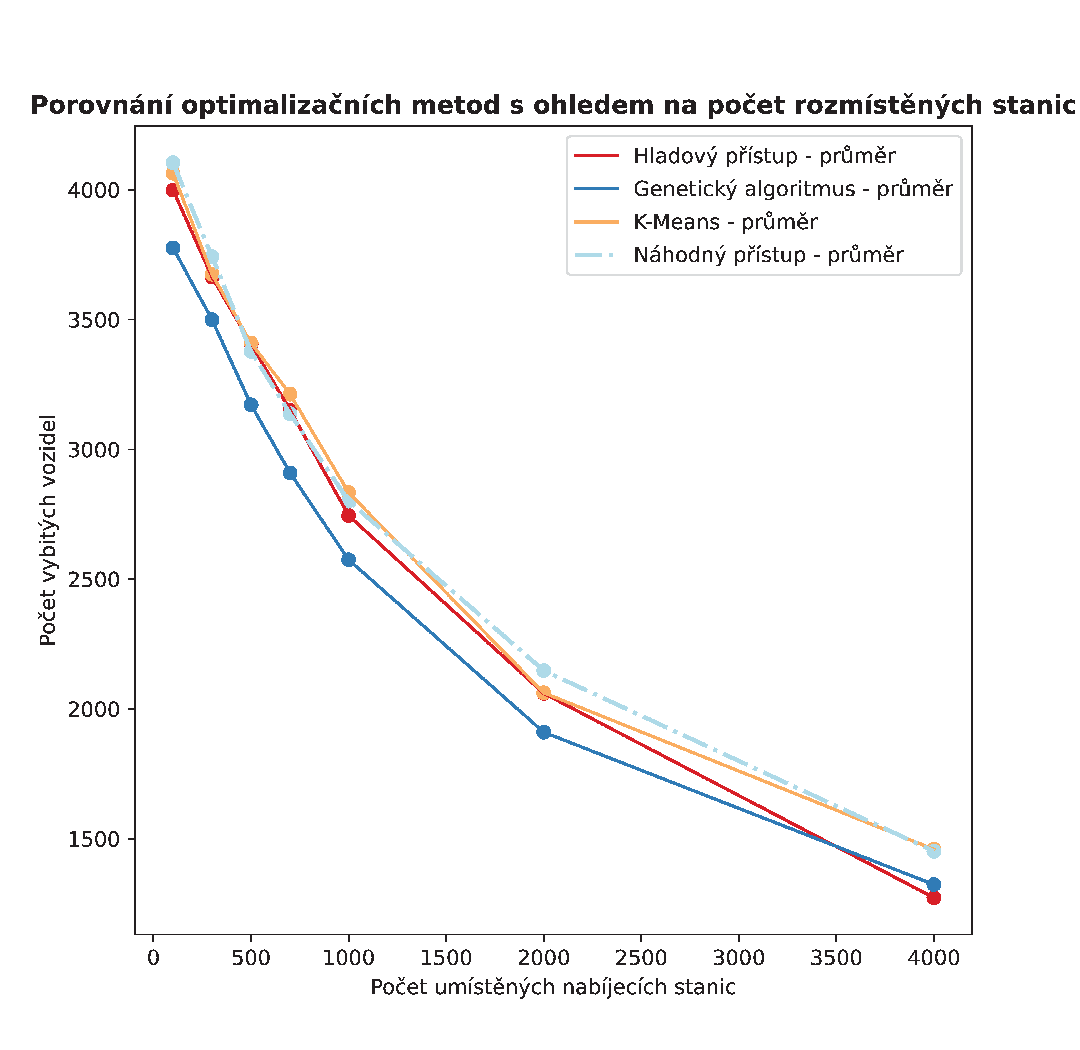
\includegraphics[width=1\linewidth]{img/all.pdf}
    \caption{Porovnání různých optimalizačních metod. Optimalizační metody barevně
    rozlišujeme. Čárové grafy popisují průměrné hodnoty počtu vybitých vozidel při
    daném počtu nabíjecích stanic umístěných v dopravní síti. 
    Čerchovaný čárový graf značí výsledky náhodného přístupu.}
    \label{fig:porovnani_optimalizaci_all}
\end{figure}


\begin{figure}
    \centering
    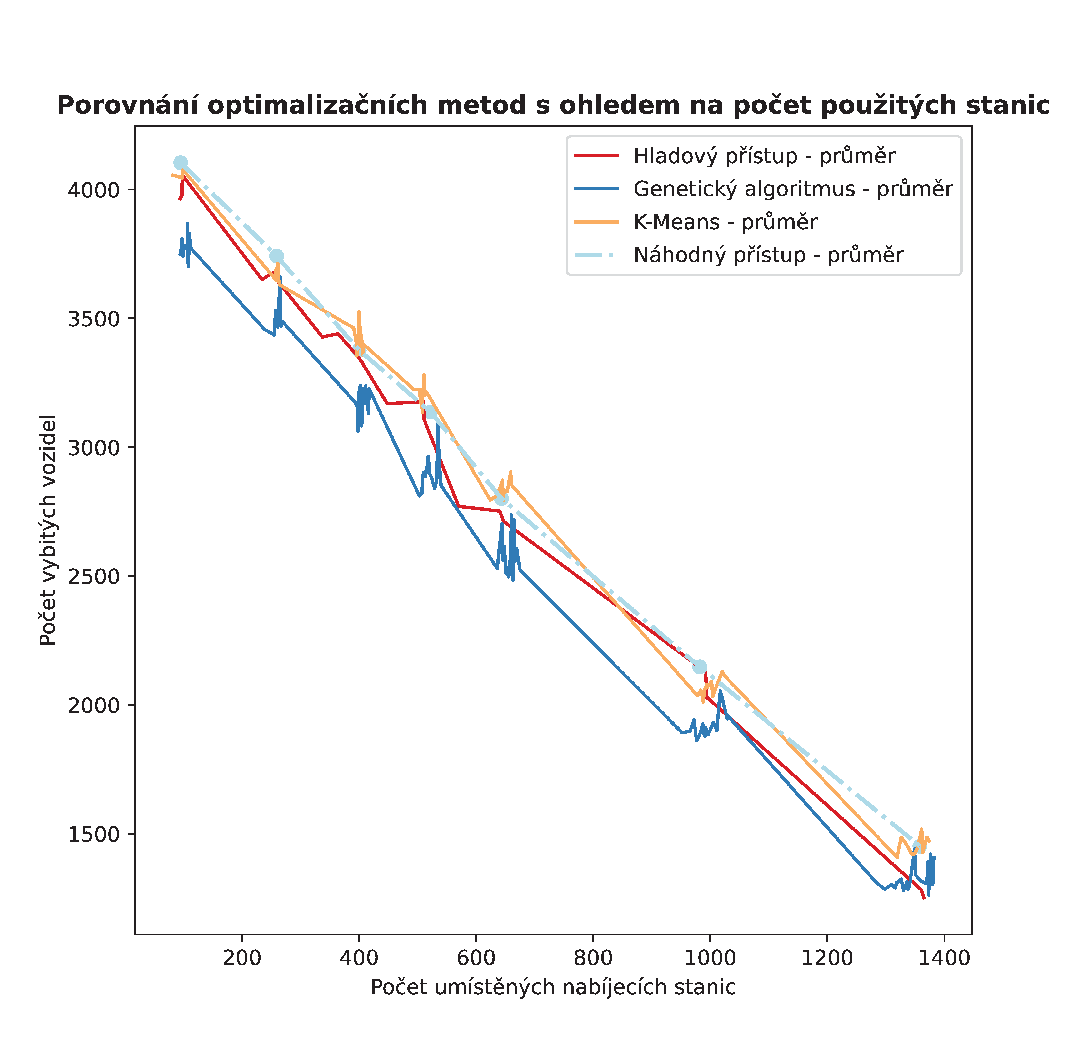
\includegraphics[width=1\linewidth]{img/used.pdf}
    \caption{Porovnání různých optimalizačních metod. Optimalizační metody barevně
    rozlišujeme. Čárové grafy popisují průměrné hodnoty počtu vybitých vozidel při
    daném počtu aspoň jednou použitých nabíjecích stanic v dopravní síti. 
    Čerchovaný čárový graf značí výsledky náhodného přístupu.}
    \label{fig:porovnani_optimalizaci_used}
\end{figure}